\documentclass{article}

\usepackage{NeededPackages}


\title{ATmega328P USART0}
\author{Narendiran S}
\date{\today}

\begin{document}
\maketitle

\section{Features}
\begin{itemize}
    \item Full duplex operation (independent serial receive and transmit registers).
    \item Asynchronous or synchronous operation
    \item High resolution baud rate generator
    \item Serial frame with 5,6,7,8,9 data bits and 1 or 2 stop bits
    \item Odd or even partiy generator and checker by hardware
    \item Double speed asynchronous communication mode
\end{itemize}
\section{Block Diagram}
\begin{figure}[H]
    \centering
    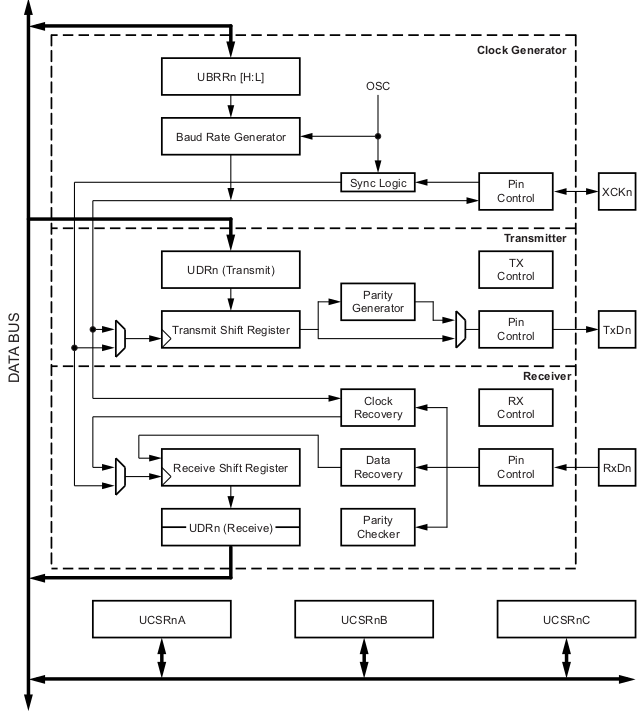
\includegraphics[height=0.58\textheight]{USART0BlockDiagram.png}
\end{figure}

\subsection{Clock Generator Block}
\begin{itemize}
    \item Consist of sync. Logic for external clock input for usage in sync. slave operation 
    \item Consist of Baud rate Generator.
    \item Uses the \pinFormat{XCKn} pin for sync. Transfer mode
\end{itemize}

\subsection{Transmitte Block}
\begin{itemize}
    \item Consist of singe write buffer – continuous transfer of data without delay between frames
    \item Consist of Serial Shift register and Parity Generator
    \item Also, Control logic for handling different serial frame format.
\end{itemize}

\subsection{Receiver Block}
\begin{itemize}
    \item Consist of Clock and data recovery unit – uses for Asynchronous reception
    \item Consist of Parity Checker, Control Logic, Shift Register, Two level Receiver buffer
    \item Can support frame error, data overrun parity error
\end{itemize}

\section{Clock Genration}
\begin{figure}[H]
    \centering
    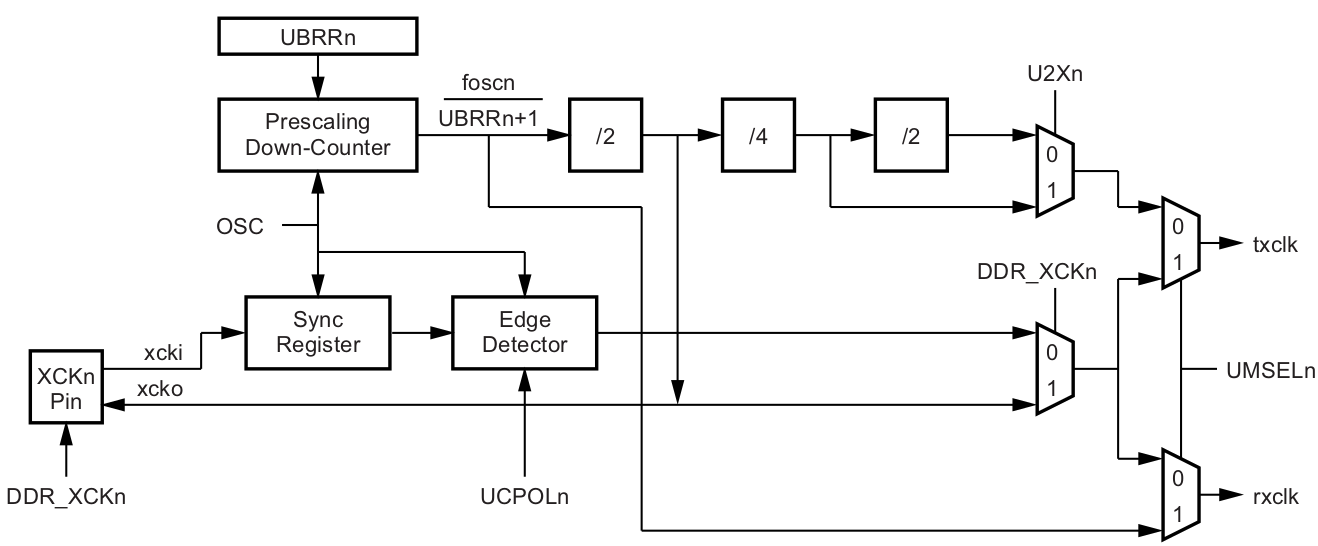
\includegraphics[width=1\textwidth]{USART0ClockGeneration.png}
\end{figure}
\begin{itemize}
    \item Generates Base Clock for Transmitter and Receiver.
    \item USART supports four modes of clock operation
    \begin{enumerate}[label=(\roman*)]
        \item Normal Asynchronous
        \item Double Speed Asynchronous
        \item Master synchronous
        \item Slave synchronous
    \end{enumerate}
    \item Selection between Asynchronous and Synchronous is done by \bitFormat{UMSELn} bit in \bitFormat{UCSRnC} - USART Control and Status Register C.
    \item The Double Speed is selected by \bitFormat{U2Xn} bit in \bitFormat{UCSRnA} - USART Control and Status Register A.
    \item In Synchronous Mode, the master or slave mode is selected by \bitFormat{DDR\_XSCn} bit direction. [external - slave mode; internal - master mode]
\end{itemize}
\begin{table}[H]
    \begin{center}
        \begin{tabular}{c|c}
            \textbf{Signals} & \textbf{Description}\\
            \hline
            txclk & Transmitte Clock\\
            rxclk & Receiver Base Clock\\
            xclki & Input from \pinFormat{XCK} pin - used for synchronous slave operation.\\
            xclko & Clock output to \pinFormat{XCK} pin - used for synchronous master operation.\\
            fosc & \pinFormat{XTAL} pin freqency (System clock).
        \end{tabular}
    \end{center}
\end{table}

\subsection{Internal Clock Generation - The Baud Rate Generator}
\begin{itemize}
    \item Used for Asynchronous and Synchronous Master modes of operation.
    \item Programmed using \regFormat{UBRRn} register.
\end{itemize}

\begin{table}[H]
    \begin{center}
        \begin{tabular}{c|c}
            \textbf{Operating Mode} & \textbf{UBRRn calculation}\\
            \hline
            Asynchronous Normal Mode(\bitFormat{U2Xn} == 0) & $UBRRn = \frac{f_{OSC}}{16 * BAUD} - 1$\\
            Asynchronous Double Speed Mode(\bitFormat{U2Xn} == 1) & $UBRRn = \frac{f_{OSC}}{8 * BAUD} - 1$\\
            Synchronous Master Mode & $UBRRn = \frac{f_{OSC}}{2 * BAUD} - 1$\\
        \end{tabular}
    \end{center}
\end{table}

\subsection{External Clock}
\begin{itemize}
    \item Used by synchronous Slave mode.
    \item External clock input from \pinFormat{XCKn} pin is used and should
\end{itemize}
\begin{center}
    $f_{XCK} < \frac{f_{OSC}}{4}$
\end{center}

\section{Frame Format}
\begin{figure}[H]
    \centering
    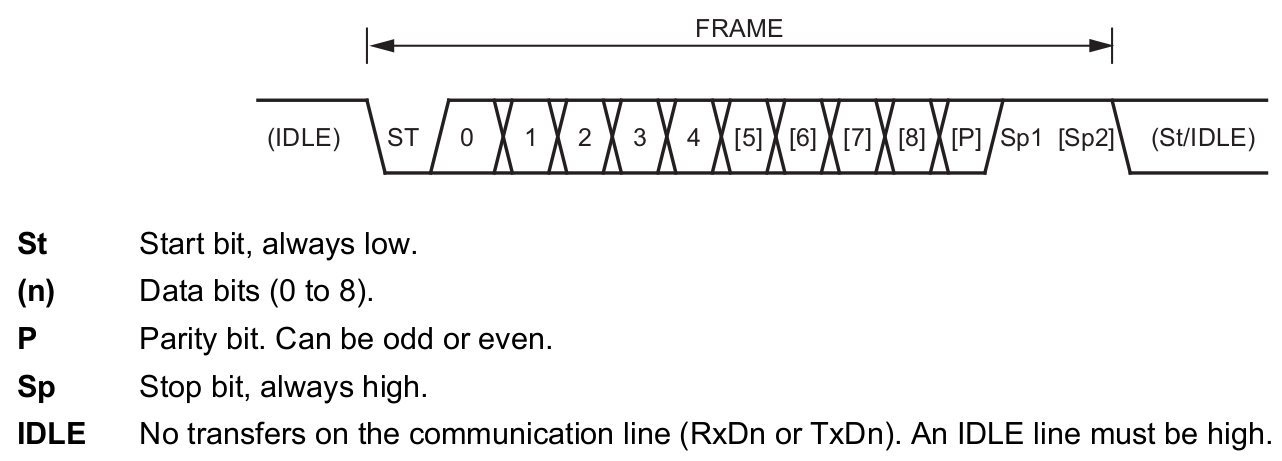
\includegraphics[width=1\textwidth]{USART0FrameFormat.png}
\end{figure}
\begin{itemize}
    \item A serial frame is defined to be one character of data bits with synchronization bits (start and stop bits), and optionally a parity bit for error checking.
    \item The combinations can be
    \begin{itemize}
        \item 1 start bit
        \item 5 or 6 or 7 or 8 or 9 data bits
        \item no or even or odd parity bits
        \item 1 or 2 stop bits
    \end{itemize}
    \item A frame starts with start bit followed by LSB data bits.
    \item Next the data bet can be from 5 to 9 ending with MSB data bits.
    \item Parity bits may be added if enabled.
    \item Finally, stop bit of 1 or 2 size is added.
    \item Generally, the line is idel with high Logic.
\end{itemize}
\section{Register Description}
\subsection*{UDRn – USART I/O Data Register n}
\vspace*{0.5cm}
\begin{bytefield}[bitformatting={\large\bfseries},
    endianness=big,bitwidth=0.125\linewidth]{8}
    \bitheader[lsb=0]{0-7} \\
    \bitbox{8}{\small RXB[7:0]}\\
    \bitbox{8}{\small TXB[7:0]}\\
\end{bytefield}

\subsubsection*{UCSRnA – USART Control and Status Register n A}
\vspace*{0.5cm}
\begin{bytefield}[bitformatting={\large\bfseries},
    endianness=big,bitwidth=0.125\linewidth]{8}
    \bitheader[lsb=0]{0-7} \\
    \bitbox{1}{\small RXCn}
    \bitbox{1}{\small TXCn}
    \bitbox{1}{\small UDREn}
    \bitbox{1}{\small FEn}
    \bitbox{1}{\small DORn}
    \bitbox{1}{\small UPEn}
    \bitbox{1}{\small U2Xn}
    \bitbox{1}{\small MPCMn}\\
\end{bytefield}
\subsubsection*{UCSRnB – USART Control and Status Register n B}
\vspace*{0.5cm}
\begin{bytefield}[bitformatting={\large\bfseries},
    endianness=big,bitwidth=0.125\linewidth]{8}
    \bitheader[lsb=0]{0-7} \\
    \bitbox{1}{\small RXCIEn}
    \bitbox{1}{\small TXCIEn}
    \bitbox{1}{\small UDRIEn}
    \bitbox{1}{\small RXENn}
    \bitbox{1}{\small TXENn}
    \bitbox{1}{\small UCSZn2}
    \bitbox{1}{\small RXBn}
    \bitbox{1}{\small TXB8n}\\
\end{bytefield}
\subsubsection*{UCSRnC – USART Control and Status Register n C}
\vspace*{0.5cm}
\begin{bytefield}[bitformatting={\large\bfseries},
    endianness=big,bitwidth=0.125\linewidth]{8}
    \bitheader[lsb=0]{0-7} \\
    \bitbox{1}{\small UMSELn1}
    \bitbox{1}{\small UMSELn0}
    \bitbox{1}{\small UPMn1}
    \bitbox{1}{\small UPMn0}
    \bitbox{1}{\small USBSn}
    \bitbox{1}{\small UCSZn1}
    \bitbox{1}{\small UCSZn0}
    \bitbox{1}{\small UCPOLn}\\
\end{bytefield}


\begin{itemize}
    \item \bitFormat{RXCn} - USART Receive Complete - Set when there are unread data in receive buffer.
    \item \bitFormat{TXCn} - USART Transmit Complete - Set when the entire frame in the transmit shift register has been shifted out and there are no new data currently present in the transmit buffer.
    \item \bitFormat{UDREn} - USART Data Register Empty - indicates if the transmit buffer is ready to receive new data. A one indicates buffer is expty and ready to transmit.
    \item \bitFormat{U2Xn} - Double the USART Transmission Speed - Affects only the asynchronous operation. One will increase the speeed of transfer rate in asynchronous opration.
    \item \bitFormat{RXCIEn} - RX Complete Interrupt Enable n - Writing one will enabled Receive Complete intterrupt.
    \item \bitFormat{TXCIEn} - TX Complete Interrupt Enable n - Writing one will enabled Transmit Complete intterrupt.
    \item \bitFormat{UDRIen} - USART Data Register Empty Interrupt Enable n - Enable data register empty intterrupt.
    \item \bitFormat{RXENn} - Receiver Enable - enable the receiever for reception.
    \item \bitFormat{TXENn} - Transmitter Enable - enable the Transmitter for Transmission.
    \item \bitFormat{UCSZn[2:0]} - Character Size n - select the number of data bits in a frame.
    \item \bitFormat{RXB8n} - Receive Data Bit 8 n - it's the actual 9th bit received.
    \item \bitFormat{TXB8n} - Transmit Data Bit 8 n -  it's the actual 9th bit to tbe trasnmitted.
    \item \bitFormat{UMSELn[1:0]} - USART Mode Select - Select the mode.
    \item \bitFormat{UPMn[1:0]} - Parity Mode - Disable or set the parity mode type.
    \item \bitFormat{USBSn} - Stop Bit select - Selects the number of stop bits to be inserted by transmitter.
\end{itemize}

\begin{table}[H]    
\begin{minipage}{0.4\linewidth}
    \begin{tabular}{c|c}
        \bitFormat{UMSELn[1:0]} & \textbf{Mode}\\
        \hline
        00 & Asynchronous USART\\
        01 & Synchronous USART\\
        10 & Reserved\\
        11 & Master SPI\\
    \end{tabular}
\end{minipage}
\begin{minipage}{0.3\linewidth}
    \begin{tabular}{c|c}
        \bitFormat{UPMn[1:0]} & \textbf{Parity Mode}\\
        \hline
        00 & Disabled\\
        01 & Reserved\\
        10 & Even Parity\\
        11 & Odd Parity\\
    \end{tabular}
\end{minipage}
\begin{minipage}{0.29\linewidth}
    \begin{tabular}{c|c}
        \bitFormat{USBSn} & \textbf{Stop Bit(s)}\\
        \hline
        0 & 1-bit\\
        0 & 2-bit\\
    \end{tabular}
\end{minipage}
\end{table}

\begin{table}[H]
    \begin{center}
        \begin{tabular}{c|c}
            \bitFormat{UCSZn[2:0]} & \textbf{Character Size}\\
            000 & 5-bit\\
            001 & 6-bit\\
            010 & 7-bit\\
            011 & 8-bit\\
            111 & 9-bit\\
        \end{tabular}
    \end{center}
\end{table}

\subsubsection*{UBRRnL and UBRRnH – USART Baud Rate Registers}
\vspace*{0.5cm}
\begin{bytefield}[bitformatting={\large\bfseries},
    endianness=big,bitwidth=0.125\linewidth]{8}
    \bitheader[lsb=8]{8-15} \\
    \bitbox{1}{\small -}
    \bitbox{1}{\small -}
    \bitbox{1}{\small -}
    \bitbox{1}{\small -}
    \bitbox{4}{\small UBRRn[11:8}\\
    \bitbox{8}{\small UBRRn[7:0}\\\\    
    \bitheader[lsb=0]{0-7} \\
\end{bytefield}

\quad \bitFormat{UBRRn[11:0]} - the actual 12-bit USART Baud Rate Registers.

\section{Configurint USART}
\begin{itemize}
    \item First, the mode is selected by confguring the \bitFormat{UMSEL0[1:0]} bits in \regFormat{UCSR0C} register.
    \item Next, the Baud rate is choosen and set in \bitFormat{UBRR0[11:0]} bits in \regFormat{UBRR0H} and \regFormat{UBRR0L} registers.
    \item Next, the frame format is set by confguring,
    \begin{itemize}
        \item Data Length - by confguring \bitFormat{UCSZ0[2:0]} bit  in \regFormat{UCSR0B} and \regFormat{UCSR0C} register.
        \item Parity - by confguring \bitFormat{UPM0[1:0]} bit  in \regFormat{UCSR0C} register.
        \item Stop bits - by confguring \bitFormat{USBS0} bit  in \regFormat{UCSR0C} register.
    \end{itemize}
    \item Interrupt may be anabled by setting bits in \bitFormat{UCSR0A} register and ISR are wirtten.
    \item Finally, the Transmitter and Receiver are enabled by setting \bitFormat{TXEN0} and \bitFormat{RXEN0} bits in \regFormat{UCSR0B}.
    \item The data can be sent by checking if the \bitFormat{UDRE0} bit is set in \regFormat{UCSR0A} register and wiring the 8-bit data into \regFormat{UDR0} register.
    \item The data can be received by checking if the \bitFormat{RXC0} bit is set in \regFormat{UCSR0A} register and reading the 8-bit data from \regFormat{UDR0} register.
    \item The code for a simple USART is seen below,
\end{itemize}

\begin{minted}[breaklines, bgcolor=lightgray]{c}
// Setting up the Mode
// Select the Asyncronous Master Mode.
// Setting UMSEL0[1:0] in UCSR0C to 00
UCSR0C &= ~(1<<UMSEL00);
UCSR0C &= ~(1<<UMSEL01);

// setting up the Buad rate
// Due to The Clock rate being 8MHz, for a buad rate of 9600
// UBRR0 = (fosc / (16*BAUD)) -1
// So UBRR0 = (8000000 / (16 * 9600)) - 1 = 0x33
UBRR0H = 0x00;
UBRR0L = 0x33;

// setting up the Frame Format
// Let's select 8-bit data bits, no parity, and 1 stop bit
// 8 - bit data bits
// By selecting UCSZ0[2:0] in UCSR0C and UCSR0B register to be 011
UCSR0B &= ~(1<<UCSZ02);
UCSR0C |= (1<<UCSZ01);
UCSR0C |= (1<<UCSZ00);
// No parity
// By selecting UPM0[1:0] in UCSR0C to 00
UCSR0C &= ~(1<<UPM01);
UCSR0C &= ~(1<<UPM00);
// 1 stop bit
// By selecting USBS0 in UCSR0C to 0 
UCSR0C &= ~(1<<USBS0);

// Disabling any interrupts
UCSR0B &= ~(1<<7);
UCSR0B &= ~(1<<6);
UCSR0B &= ~(1<<5);

// Enabling Transmitter 
UCSR0B |= (1<<TXEN0);
// Enabling Receiver
UCSR0B |= (1<<RXEN0);
\end{minted}

\begin{minted}[breaklines, bgcolor=lightgray]{c}
void USART0sendChar(uint8_t data_)
{
	//cHECKING if transmitet buffer is empty
	while((UCSR0A & (1<<UDRE0)) == 0x00){};		
	UDR0 = data_;	
}
uint8_t USART0receiveChar()
{
	// wait for thedate to be recied
	while((UCSR0A & (1<<RXC0)) == 0x00){};		
	return UDR0;
}
\end{minted}

\end{document}